\documentclass[12pt,a5paper]{book}
\usepackage[utf8]{vietnam}
\usepackage{amsmath}
\usepackage{amsfonts}
\usepackage{tikz}
\usepackage{amssymb}
\usepackage{graphicx}
\usepackage{listings}
\usepackage{textcomp}
\usepackage{hyperref}
\renewcommand{\familydefault}{\sfdefault}
\usepackage[left=2cm,right=1.5cm,top=1.5cm,bottom=1.5cm]{geometry}

 \renewcommand\lstlistingname{Quelltext} % Change language of section name

\lstset{ % General setup for the package
	language=C,
	basicstyle=\small\sffamily,
	numbers=left,
 	numberstyle=\tiny,
	frame=tb,
	tabsize=4,
	columns=fixed,
	showstringspaces=false,
	showtabs=false,
	keepspaces,
	%commentstyle=\color{green},
	%keywordstyle=\color{blue}
}
\pagenumbering{gobble}
\pagenumbering{arabic}
\title{LẬP TRÌNH NHÚNG}
\author{Nguyễn Thành Công}


\begin{document}
\maketitle
\begin{figure}
\centering
 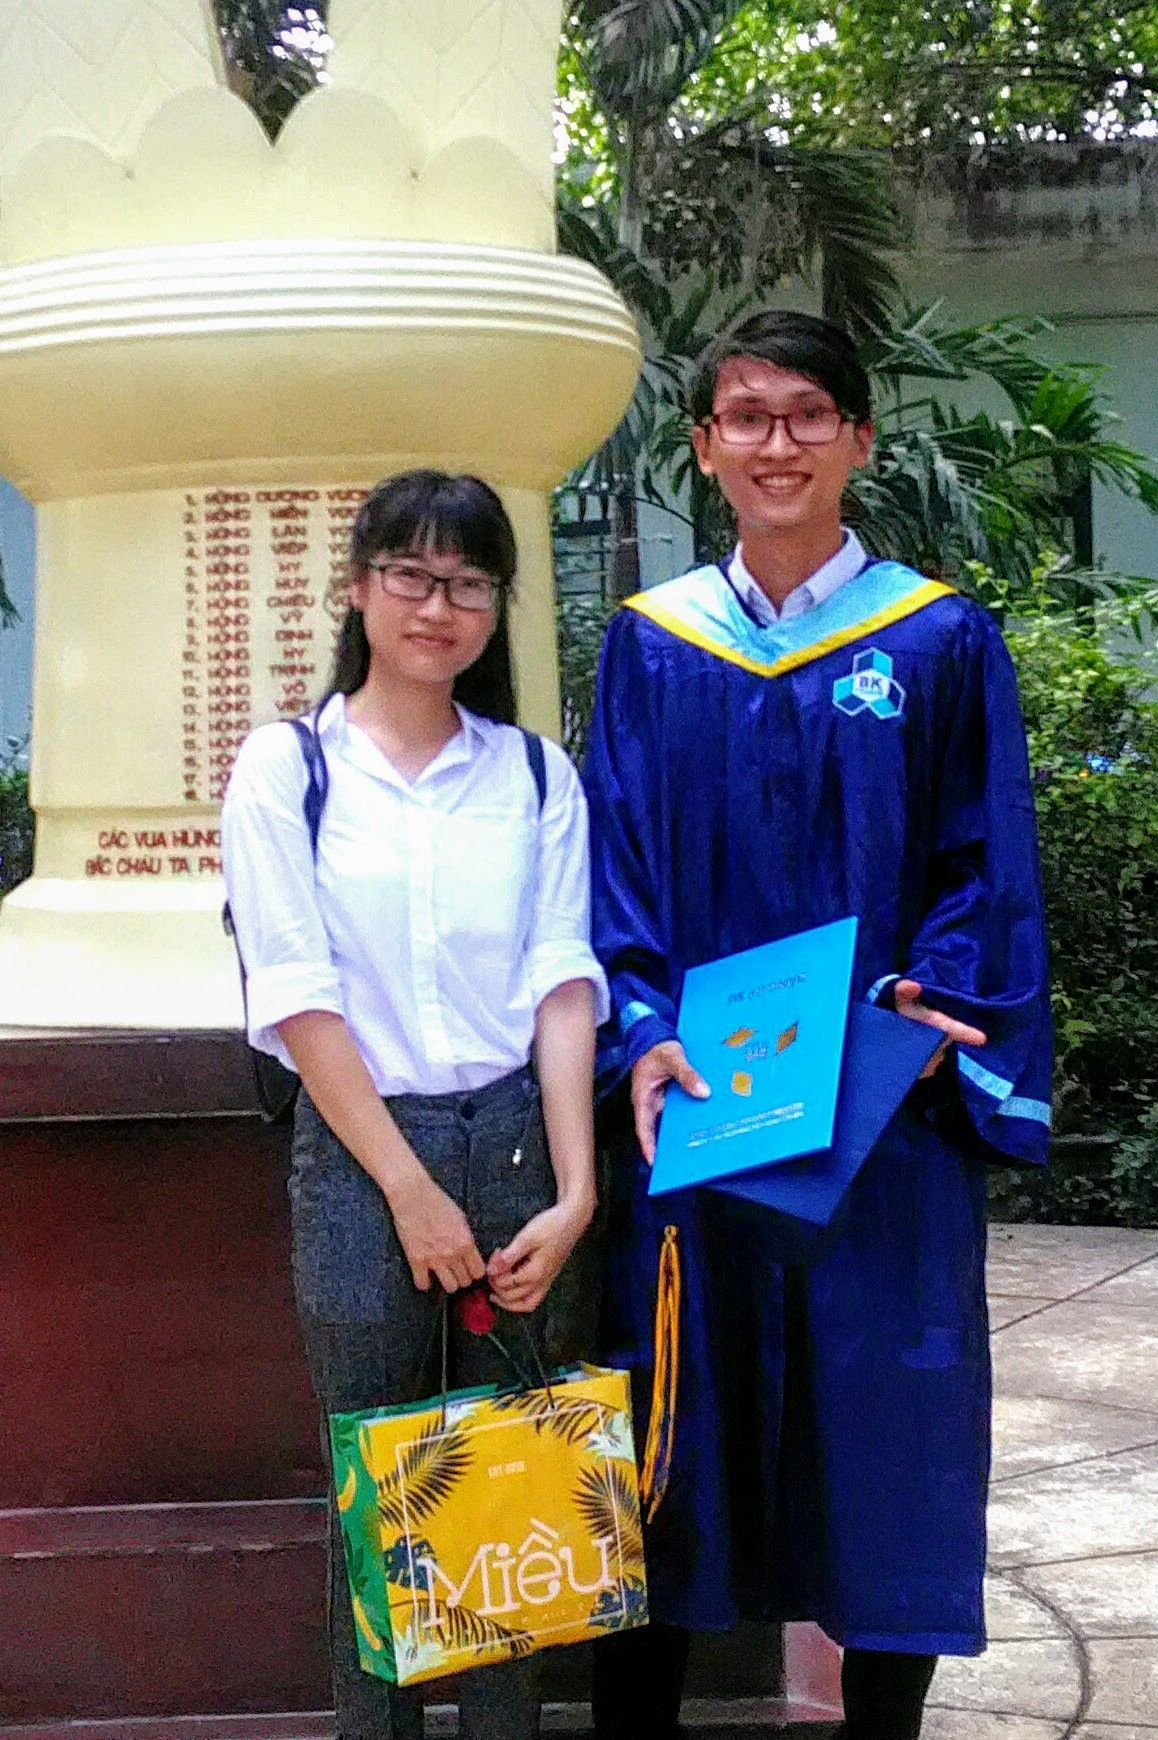
\includegraphics[width=0.5\linewidth]{tao.jpg}
 \caption{Tui}
\end{figure}
\tableofcontents{}
 \chapter{Chém gió xíu }
	\section{Về lập trình nhúng}
		\paragraph{}
Đặc trưng của lập trình nhúng là viết chương trình để điều khiển phần cứng, ví dụ như chương trình điều khiển động cơ bước chẳng hạn. Với phần mềm ứng dụng như trên máy tính mà phần cứng yêu cầu giống nhau (màn hình, chuột, cpu...) và đòi hỏi nặng về khả năng tính toán của cpu. Còn với chương trình nhúng thì phần cứng của nó cực kì đa dạng, khác nhau với mỗi ứng dụng như chương trình điều khiển động cơ hoặc chương trình đọc cảm biến, nó không đòi hỏi cpu phải tính toán quá nhiều, chỉ cần quản lý tốt phần cứng bên dưới. 
		\paragraph{}
Có 2 khái niệm là Firmware, ý chỉ chương trình nhúng, và Software, chương trình ứng dụng trên máy tính, được đưa ra để người lập trình dễ hình dung, nhưng không cần thiết phải phân biệt rõ ràng.
		\paragraph{}
Khi lập trình hệ thống nhúng, việc biết rõ về phần cứng là điều cần thiết. Bởi bạn phải biết phần cứng của mình như thế nào thì bạn mới điều khiển hoặc quản lí tốt nó được. Tốt nhất là làm trong team hardware một thời gian rồi nhảy qua team firmware, hoặc làm song song cả hai bên (nếu bạn đủ sức).
		\paragraph{}
Tóm lại: \textit{Lập trình nhúng là viết chương trình điều khiển phần cứng, bạn phải biết lập trình, và phải giỏi về phần cứng.} 
	\section{Về ngôn ngữ C trong lập trình nhúng}
		\paragraph{}
	Ngôn ngữ C cho phép tương tác rất mạnh tới phần cứng, mạnh thế nào thì hồi sau sẽ rõ, thế nên nó thường được lựa chọn trong các dự án lâp trình nhúng. Ngoài ra có thể dùng C++ và Java nhưng mình ít xài chúng nên không đề cập ở đây.
		\paragraph{}
	Việc học C cơ bản mình sẽ không đề cập tới vì tài liệu nó nhiều lắm, các bạn có để xem và làm vài bài tập sử dụng được ngôn ngữ này. Lưu ý là ranh giới giữa việc Biết và Sử Dụng Được ngôn ngữ C là việc bạn có làm bài tập hay không nhé. Về cú pháp thì nó quanh đi quẩn lại chỉ là khai báo biến, rồi mấy vòng lặp for, while hoặc rẽ nhánh if, else chẳng hạn, nhưng Kỹ Năng sử dụng C để giải quyết một vấn đề thì cần nhiều bài tập để trau dồi.
		\paragraph{}
	Tóm lại: \textit{bạn không thể đọc sách học bơi là biết bơi, không thể đọc kiếm phổ là thành cao thủ.}
	\section{Về phần cứng để demo}
	Trong phần này mình sẽ sử dụng kit STM32F4 Discovery để thực hành, ngoài ra phần thiên về lập trình không cần phần cứng sẽ sử dụng chương trình DevC++, những cái cơ bản các bạn nên tự tìm hiểu nhé, vì những cái đó tài liệu nó rất nhiều, và bạn cũng có thể tự mò để thể hiện bản lĩnh.
	\section{Về Tiếng Anh, vâng Tiếng Anh...}
		\paragraph{}
	Mấy ngành khác thì mình không rành chứ mà làm nhúng mà bạn không biết Tiếng Anh là tự níu chân mình lại. Vì mỗi linh kiện điện tử đều kèm theo một cái bảng thông tin đặc tính là datasheet, cái nào phức tạp thì sẽ kèm theo một cái hướng dẫn sử dụng là user manual. Và tất nhiên 96.69\% chúng được viết bằng tiếng anh, còn lại là tiếng Trung Quốc. Và tin buồn là code trong lập trình nhúng đều biết bằng tiếng anh, tin buồn hơn nữa là tài liệu, sách hướng dẫn, các diễn đàn sử dụng Tiếng Anh rất nhiều và nhiều cái rất hay.
		\paragraph{}
	Tóm lại là không biết nó thì công việc của bạn bị cản trở rất nhiều, phụ thuộc rất nhiều vào google dịch củ chuối. Hãy dừng một bước để học tiếng anh và tiến 3 bước trong con đường sự nghiệp. Chí ít bạn phải đọc được datasheet mà không cần tra quá nhiều từ, đọc được cuốn sách như clean code chẳng hạn, hoặc viết email cho thằng bán linh kiện ở Trung Quốc vì kiểu gì sau này bạn cũng đặt hàng ở bên đó.
		\paragraph{}
	\textit{Nhớ rằng tiếng Anh là công cụ để sử dụng. Như người ta học đi xe máy để đi lại nhanh hơn. Hãy học tiếng Anh để làm việc ngon lành hơn.}


	\chapter{Ngôn ngữ C trong lập trình nhúng}
	\paragraph{}
Hãy nhớ là bạn làm vài bài tập về ngôn ngữ C rồi hãy đọc phần này nhé.
	\paragraph{}
Có cuốn sách hay mà bạn có thể kiếm là Nhập Môn Lập Trình của trường Khoa Học Tự Nhiên (sách bìa màu đen ấy).\\
	\section{Cơ bản về chương trình.}
	\paragraph{} 
Đại khái thì việc lập trình là chỉ cho cái máy biết bạn muốn nó làm cái gì.
	\paragraph{}
Khi bạn viết chương trình, bên dịch thì máy tính sẽ biên dịch code của bạn (người hiểu được) thành mã máy (máy hiểu được) bao gồm các lệnh mà vi điều khiển sẽ thực và khi nạp xuống cho vi điều khiển thì chương trình sẽ được lưu ở ROM (bộ nhớ chương trình). CPU sẽ đọc lệnh từ bộ nhớ chương trình rồi thực thi. Lưu ý là CPU chỉ đọc thôi nhé, nó không được phép ghi gì vào bộ nhớ chương trình. Nó không thể cãi lệnh bạn! Thế nên bộ nhớ chương trình có tên là bộ nhớ chỉ đọc (Read-only memory, ROM). Nó vẫn còn đấy khi mất điện.
	\paragraph{}
Còn bộ nhớ RAM là để phục vụ cho chương trình được thực thi.
	\paragraph{}
Ví dụ như bạn khai báo biến int a=0; thì biến a sẽ được lưu trong RAM. Sau đó có lệnh a=a+1; CPU sẽ lấy biến a từ trong RAM ra, thực hiện phép tính rồi lại lưu vào chỗ cũ.
	\paragraph{}
Do việc RAM được CPU sử dụng để thực hiện chương trình, đọc ghi liên tục nên nó gọi là bộ nhớ truy cập ngẫu nhiên (Random-access Memory) hay nói cách khác CPU đươc toàn quyền sử dụng bộ nhớ RAM (không như việc chỉ được quyền đọc từ ROM thôi nhé).



	\section{Về cách tổ chức bộ nhớ}
	\paragraph{}
	Thông thường thì đơn vị nhỏ nhất của bộ nhớ là byte (mà mình hay gọi là ô nhớ), mỗi byte đươc đánh một địa chỉ. Nếu vi xử lý 8-bit thì nó có thể quản lý 256 byte bộ nhớ, vi xử lý 16-bit thì có thể quản lý 64kbyte, còn 32-bit thì có thể quản lý tới 4Gbyte bộ nhớ. 
	
\begin{figure}[h!]
	\centering
	
	%\label{fig:Bộ nhớ 16 bit}
	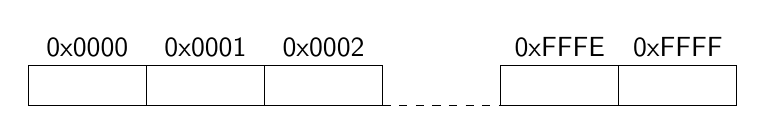
\begin{tikzpicture}[yscale=0.5, xscale=1.5]

		\draw (0,0) rectangle (1,1);
		\draw (1,0) rectangle (2,1);
		\draw (2,0) rectangle (3,1);
		\draw [dashed] (3,0) -- (4,0);
		\draw (4,0) rectangle (5,1);
		\draw (5,0) rectangle (6,1);
		\node  [above] at (0.5, 1) {0x0000};
		\node  [above] at (1.5, 1) {0x0001};
		\node  [above] at (2.5, 1) {0x0002};
		\node  [above] at (4.5, 1) {0xFFFE};
		\node  [above] at (5.5, 1) {0xFFFF};
	\end{tikzpicture}
	\caption{Bộ nhớ địa chỉ 16-bit} 
\end{figure}

	Vậy mỗi ô nhớ sẽ có 2 thông số mà bạn cần quan tâm: địa chỉ (nó ở đâu, địa chỉ có thể là số 8-bit, 16-bit, 32-bit...), và giá trị được lưu (nó bao nhiêu, chỉ là số 8-bit (1 byte) thôi nhé).
	
	\begin{figure}[h!]
	\centering
	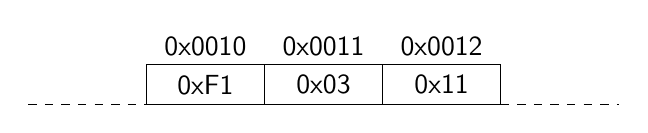
\begin{tikzpicture}[yscale=0.5, xscale=1.5]
		\draw [dashed] (0,0) -- (1,0);
		\draw (1,0) rectangle (2,1);
		\draw (2,0) rectangle (3,1);
		\draw (3,0) rectangle (4,1);
		\draw [dashed] (4,0) -- (5,0);
		
		\node  [above] at (1.5, 1) {0x0010};
		\node  [above] at (2.5, 1) {0x0011};
		\node  [above] at (3.5, 1) {0x0012};
		\node   at (1.5, 0.5) {0xF1};
		\node   at (2.5, 0.5) {0x03};
		\node   at (3.5, 0.5) {0x11};

	\end{tikzpicture}
	\caption{Dữ liệu trong bộ nhớ} %\label{fig: Dữ liệu trong bộ nhớ}
\end{figure}

	\paragraph{}
	Chip STM32 là vi điều khiển 32-bit nhưng nó chỉ có vài kbyte bộ nhớ RAM nên dãy địa chỉ RAM có thể được đánh dấu từ 0x00000000 đến 0x0000FFFF chẳng hạn. Nếu bạn muốn ghi vào địa chỉ 0xF0000000 thì nó sẽ biến mất hoặc báo lỗi không biết trước được.
	\paragraph{}
	Đoạn chương trình để xem địa chỉ trong DevC++:\*
\begin{lstlisting}
	#include <stdio.h>
	void main(){
		char a;
		printf("a address: 0x%08x\n", &a);
	}
\end{lstlisting}

	
	\section{Khai báo biến}
	\paragraph{}
Các kiểu biến thông thường khi lập trình C là char, int, long, float double. Nhưng trong lập trình nhúng, tài nguyên bộ nhớ hạn chế nên việc bạn biết các biến chiếm bao nhiêu ô nhớ là điều rất quan trọng. Thông thường, các biến được khai báo dưới dạng uint8\_t, int8\_t, uint16\_t, int16\_t... để sử dụng thì bạn cần  \#include <stdint.h>. Đoán xem mỗi kiểu sẽ chiếm bao nhiêu ô nhớ, và kiểu nào là kiểu có dấu, không đấu?
	\paragraph{}
	Một điểm đặc biệt là kiểu uint8\_t thường được dùng để đại diện cho một ô nhớ (8-bit). Ví dụ khi khai báo uint8\_t array[3], thì có thể hiểu là khai báo 3 phần tử mảng array có kiểu là uint8\_t, hoặc cũng có thể hiểu là yêu cầu bộ nhớ cấp 3 ô nhớ kề nhau. Việc này thường được dùng để khai báo các bộ đệm trong các giao tiếp như uart, i2c, spi...
	\paragraph{}
	Thế nên hãy thường sử dụng các kiểu dữ liệu với bộ nhớ tường minh trên để kiểm soát bộ nhớ chặt chẽ hơn.\\
\section{Kiểu dữ liệu tự định nghĩa}
\paragraph{}
Ngôn ngữ C cung cấp cơ chế tự định nghĩa kiểu dữ liệu để việc truy xuất dữ liệu được thuận tiện.

\paragraph{}
Ví dụ mình có một cái cảm biến có thể đọc về nhiệt độ, độ ẩm và ánh sáng môi trường. Dữ liệu nhiệt độ từ  -20\textdegree{}C đến 100\textdegree{}C, độ ẩm từ 0\% đến 100\%, ánh sáng từ 0 lux đến 50.000 lux. Vậy mình khai báo dữ kiểu dữ liệu env\_t (environment type) như sau: 
\begin{lstlisting}
	typedef struct{
		int8_t temp;
		uint8_t humi;
		uint16_t lux;
	}env_t;
\end{lstlisting}
\paragraph{}
Dễ thấy là các kiểu biến bên trong đều chứa đủ khoảng giá trị cần thiết (nếu nhiệt độ vượt quá 127\textdegree{}C thì biến int8\_t không chứa nổi nhé.
\paragraph{}
Thực chất kiểu dữ liệu là cách bạn tương tác với một vùng nhớ cho trước. Ví dụ khi khai báo một biến như env\_t evn; chẳng hạn, nó sẽ cung cấp cho bạn 4 ô nhớ liền nhau. Nếu bạn in địa chỉ của biến env ra nó sẽ hiển thị địa chỉ ô nhớ \textit{đầu tiên} của dãy 4 ô nhớ đó. Và kiểu env\_t sẽ cho máy tính biết cách truy cập tới 4 ô nhớ đó như thế nào.

\begin{figure}[h!]
	\centering
	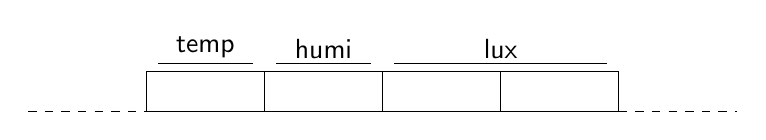
\begin{tikzpicture}[yscale=0.5, xscale=1.5]
		\draw [dashed] (0,0) -- (1,0);
		\draw (1,0) rectangle (2,1);
		\draw (2,0) rectangle (3,1);
		\draw (3,0) rectangle (4,1);
		\draw (4,0) rectangle (5,1);
		\draw [dashed] (5,0) -- (6,0);
		
		\draw (1.1, 1.2) -- (1.9, 1.2);
		\node [above] at (1.5, 1.1) {temp};
		
		\draw (2.1, 1.2) -- (2.9, 1.2);
		\node [above] at (2.5, 1.1) {humi};
		
		\draw (3.1, 1.2) -- (4.9, 1.2);
		\node [above] at (4, 1.1) {lux};
		
	\end{tikzpicture}
	\caption{Truy cập biến kiểu env\_t} %\label{fig: Dữ liệu trong bộ nhớ}
\end{figure}
\paragraph{}
Đoạn chương trình xem độ dài của kiểu dữ liệu:
\begin{lstlisting}
#include <stdio.h>
#include <stdint.h>

typedef struct{
	int8_t temp;
	uint8_t humi;
	uint16_t lux;
}env_t;

void main(void) {
	printf("Size of env_t: %d\n", sizeof(env_t));
}
\end{lstlisting}
\paragraph{}
Một điểm cần lưu ý là các máy tính thường có cơ chế làm tròn biên kiểu dữ liệu (data structure alignment). Nếu chúng ta khai báo như sau:

\begin{lstlisting}
typedef struct{
	int8_t temp;
	uint16_t lux;
	uint8_t humi;
}env_t;
\end{lstlisting}
biến lux khai báo ở giữa, thì kiểu dữ liệu env\_t giờ đây có độ dài là 6 byte chứ không phải 4!!!.
\paragraph{}
Kiểu biến env\_t giờ có cấu trúc như sau:
\begin{figure}[h!]
	\centering
	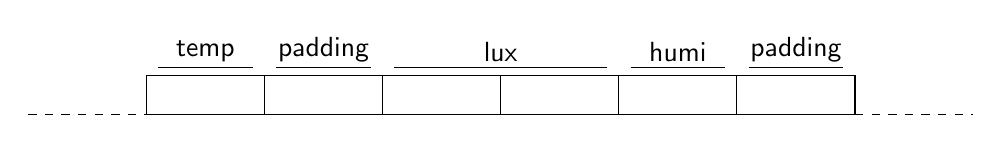
\begin{tikzpicture}[yscale=0.5, xscale=1.5]
		\draw [dashed] (0,0) -- (1,0);
		\draw (1,0) rectangle (2,1);
		\draw (2,0) rectangle (3,1);
		\draw (3,0) rectangle (4,1);
		\draw (4,0) rectangle (5,1);
		\draw (5,0) rectangle (6,1);
		\draw (6,0) rectangle (7,1);
		\draw [dashed] (7,0) -- (8,0);
		
		\draw (1.1, 1.2) -- (1.9, 1.2);
		\node [above] at (1.5, 1.1) {temp};
		
		\draw (2.1, 1.2) -- (2.9, 1.2);
		\node [above] at (2.5, 1.1) {padding};
		
		\draw (3.1, 1.2) -- (4.9, 1.2);
		\node [above] at (4, 1.1) {lux};
		
		\draw (5.1, 1.2) -- (5.9, 1.2);
		\node [above] at (5.5, 1.1) {humi};
		
		\draw (6.1, 1.2) -- (6.9, 1.2);
		\node [above] at (6.5, 1.1) {padding};
	\end{tikzpicture}
	\caption{Truy cập biến kiểu env\_t} %\label{fig: Dữ liệu trong bộ nhớ}
\end{figure}
\paragraph{}
Hai ô nhớ tên padding được thêm vào để tăng hiệu suất việc đọc ghi dữ liệu trong máy tính hiện đại. Các bạn quan tâm thì có thể tìm hiểu thêm. Ta có thể tránh nó bằng cách khai báo như sau: trong DevC++ thì bạn khai báo \textit{\#pragma pack(1)} trước khi khai báo biến dữ liệu, còn trong KeilC thì khai báo kiểu:

\begin{lstlisting}
typedef __packed struct{
	int8_t temp;
	uint16_t lux;
	uint8_t humi;
}env_t;
\end{lstlisting}
mỗi khi khai báo một kiểu biến nào đó.

\paragraph{}
Ngoài ra còn một số kiểu enum và union mà các bạn hỏi giáo sư gu gồ hen.

\section{Con trỏ}
\paragraph{}
Có thể nói con trỏ là công cụ lợi hại nhất của C, bạn khó mà giỏi C nếu bỏ qua con trỏ được. Bản chất của con trỏ (chưa nói đến con trỏ hàm) là trỏ tới một vùng nhớ nào đó và tương tác với vùng nhớ đó. Chương trình ví dụ về con trỏ:
\begin{lstlisting}
#include <stdio.h>
#include <stdint.h>

int main(void) {
	uint16_t a=0;
	uint16_t *pa;
	pa=&a;
	printf("a addr: 0x%08x\n", &a);
	printf("a addr: 0x%08x\n", pa);
}
\end{lstlisting}

hai lần printf sẽ cho ra kết quả như nhau vì đã gán địa chỉ của a cho pa.
\paragraph{}
Lưu ý là bạn không cần quan tâm địa chỉ thật của a (có dạng số hex như 0x0012) chỉ cần khai báo biến a, nó sẽ nằm đâu đó trong RAM (nếu RAM còn trống) và có phép lấy địa chỉ \&a.

\end{document}
